\documentclass[12pt,a4paper]{standalone}
\usepackage{amssymb}
\usepackage{amsmath}
\usepackage{bm}
\usepackage{tikz}
\usetikzlibrary{arrows.meta}
\usetikzlibrary{arrows}
\usepackage{pstricks}
\usetikzlibrary{patterns}
\usetikzlibrary{fadings}
\usetikzlibrary{shapes.geometric}







\begin{document}
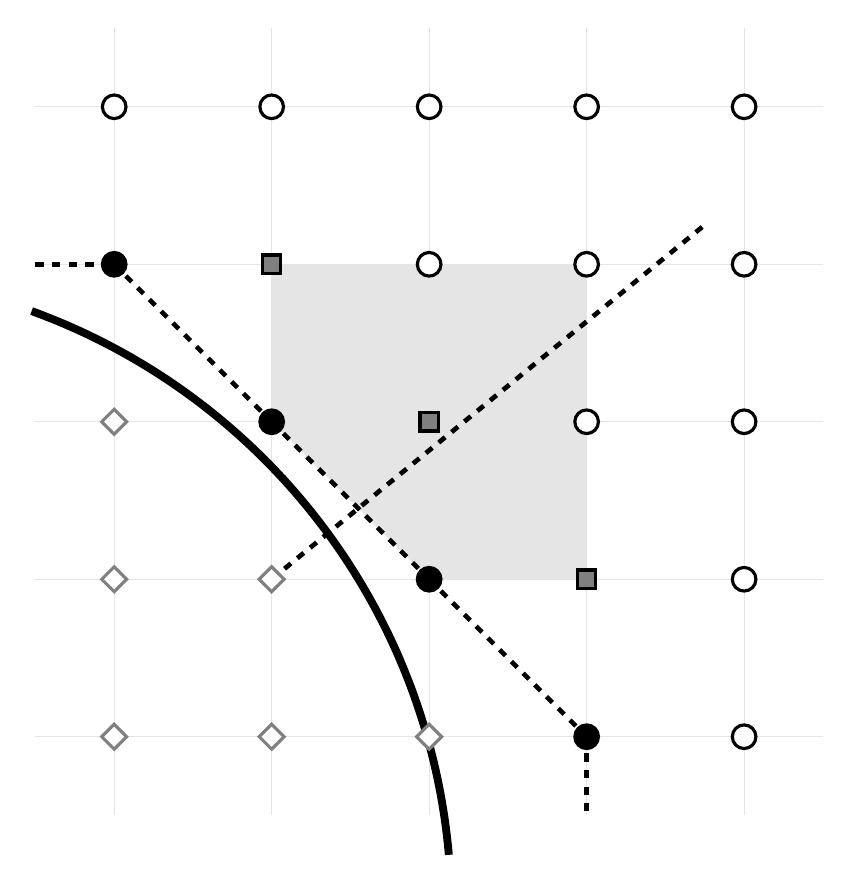
\begin{tikzpicture}[line width=0.4mm][>=Latex]
%\draw[dashed,thick,line width=0.6mm] (4,2) -- (7.7,7.4);

\fill[black!10] (6,4) rectangle (8,6);
\fill[black!10] (8,4) rectangle (10,6);
\fill[black!10] (8,4) -- (8,2) -- (6,4) -- cycle;
\fill[black!10] (8,2) rectangle (10,4);

\draw[gray!20,solid,thick,line width=0.1mm] (3,0) -- (13,0);
\draw[gray!20,solid,thick,line width=0.1mm] (3,2) -- (13,2);
\draw[gray!20,solid,thick,line width=0.1mm] (3,4) -- (13,4);
\draw[gray!20,solid,thick,line width=0.1mm] (3,6) -- (13,6);
\draw[gray!20,solid,thick,line width=0.1mm] (3,8) -- (13,8);

%\draw[gray!20,solid,thick,line width=0.1mm] (2,-1) -- (2,9);
\draw[gray!20,solid,thick,line width=0.1mm] (4,-1) -- (4,9);
\draw[gray!20,solid,thick,line width=0.1mm] (6,-1) -- (6,9);
\draw[gray!20,solid,thick,line width=0.1mm] (8,-1) -- (8,9);
\draw[gray!20,solid,thick,line width=0.1mm] (10,-1) -- (10,9);
\draw[gray!20,solid,thick,line width=0.1mm] (12,-1) -- (12,9);

\draw[thick,line width=1mm] (8.25,-1.5) arc[start angle=5, end angle=70, radius=8.1];
\draw[dashed,thick,line width=0.6mm] (6,2) -- (11.5,6.5);


\draw[dashed,thick,line width=0.6mm] (3,6) -- (4,6);
\draw[dashed,thick,line width=0.6mm] (4,6) -- (6,4);
\draw[dashed,thick,line width=0.6mm] (6,4) -- (8,2);
\draw[dashed,thick,line width=0.6mm] (8,2) -- (10,0);
\draw[dashed,thick,line width=0.6mm] (10,0) -- (10,-1);


%top first row
%\draw[black,fill=white] (2,8)node[]{} circle(0.15cm);
\draw[black,fill=white] (4,8)node[]{} circle(0.15cm);
\draw[black,fill=white] (6,8)node[]{} circle(0.15cm);
\draw[black,fill=white] (8,8)node[]{} circle(0.15cm);
\draw[black,fill=white] (10,8)node[]{} circle(0.15cm);
\draw[black,fill=white] (12,8)node[]{} circle(0.15cm);

%top second row

%\draw[black,fill=black] (2,6)node[]{} circle(0.15cm);
\draw[black,fill=black] (4,6)node[]{} circle(0.15cm);
\node[draw, black, fill=gray, rectangle, minimum size=0.2cm] at (6,6) {};
%\draw[black,fill=white] (6,6)node[]{} circle(0.15cm);
\draw[black,fill=white] (8,6)node[]{} circle(0.15cm);
\draw[black,fill=white] (10,6)node[]{} circle(0.15cm);
\draw[black,fill=white] (12,6)node[]{} circle(0.15cm);

\def\rstart{0.18}   % distance from center
\def\rlen{1.6}      % arrow length

%\draw[black, thick, {Latex}-]
%(8,4) ++(\rstart,0) -- ++(\rlen,0)
%node[midway,below, yshift=2pt,font=\fontsize{14pt}{12pt}\selectfont] {$c_3$};
%
%% up (2)
%\draw[black, thick, {Latex}-]
%(8,4) ++(0,\rstart) -- ++(0,\rlen)
%node[midway, left, xshift=4pt,font=\fontsize{14pt}{12pt}\selectfont] {$c_4$};
%
%% left (3)
%\draw[black, thick, {Latex}-]
%(8,4) ++(-\rstart,0) -- ++(-\rlen,0)
%node[midway, below, yshift=2pt,font=\fontsize{14pt}{12pt}\selectfont] {$c_1$};
%
%% down (4)
%\draw[black, thick, {Latex}-]
%(8,4) ++(0,-\rstart) -- ++(0,-\rlen)
%node[midway, left, xshift=4pt,font=\fontsize{14pt}{12pt}\selectfont] {$c_2$};
%
%% diagonals
%\draw[black, thick, {Latex}-]
%(8,4) ++(\rstart,\rstart) -- ++(\rlen,\rlen)
%node[midway, above right,xshift=-4pt, yshift=7pt,font=\fontsize{14pt}{12pt}\selectfont] {$c_7$};
%
%\draw[black, thick, {Latex}-]
%(8,4) ++(\rstart,-\rstart) -- ++(\rlen,-\rlen)
%node[midway, below right,xshift=-4pt, yshift=-7pt,font=\fontsize{14pt}{12pt}\selectfont] {$c_6$};
%
%\draw[black, thick, {Latex}-]
%(8,4) ++(-\rstart,\rstart) -- ++(-\rlen,\rlen)
%node[midway, above left,xshift=4pt, yshift=7pt,font=\fontsize{14pt}{12pt}\selectfont] {$c_8$};





%top third row
%\draw[black,fill=white] (2,4)node[]{} circle(0.15cm);
\node [draw, gray, fill=white,diamond, aspect=1,scale=0.7] at (4,4) {};

\draw[black,fill=black] (6,4)node[]{} circle(0.15cm);
\node[draw, black, fill=gray, rectangle, minimum size=0.2cm] at (8,4) {};
%\draw[black,fill=black] (8,4)node[]{} circle(0.15cm);
\draw[black,fill=white] (10,4)node[]{} circle(0.15cm);
\draw[black,fill=white] (12,4)node[]{} circle(0.15cm);

%top fourth row
%\node [draw, gray, fill=white,diamond, aspect=1,scale=0.7] at (2,2) {};
\node [draw, gray, fill=white,diamond, aspect=1,scale=0.7] at (4,2) {};
\node [draw, gray, fill=white,diamond, aspect=1,scale=0.7] at (6,2) {};
\draw[black,fill=black] (8,2)node[]{} circle(0.15cm);
\node[draw, black, fill=gray, rectangle, minimum size=0.2cm] at (10,2) {};
%\draw[black,fill=white] (10,2)node[]{} circle(0.15cm);
\draw[black,fill=white] (12,2)node[]{} circle(0.15cm);

%top fifth row
%\node [draw, gray, fill=white,diamond, aspect=1,scale=0.7] at (2,0) {};
\node [draw, gray, fill=white,diamond, aspect=1,scale=0.7] at (4,0) {};
\node [draw, gray, fill=white,diamond, aspect=1,scale=0.7] at (6,0) {};
\node [draw, gray, fill=white,diamond, aspect=1,scale=0.7] at (8,0) {};
\draw[black,fill=black] (10,0)node[]{} circle(0.15cm);
\draw[black,fill=white] (12,0)node[]{} circle(0.15cm);





%\tikzset{myblue/.style={draw=blue, fill=white, line width=0.5mm, circle, minimum size=0.3cm, inner sep=0pt}}
%
%% Boundary nodes with labels p1, p2, ...
%\tikzset{mydot/.style={draw=black, fill=red, line width=0mm, circle, minimum size=0.35cm, inner sep=0pt}}
%
%%Bc fluid
%\tikzset{myblue2/.style={draw=blue, fill=blue, line width=0.5mm, circle, minimum size=0.3cm, inner sep=0pt}}
%\tikzset{mygray/.style={draw=gray!30, fill=gray!30, line width=0.5mm, circle, minimum size=0.25cm, inner sep=0pt}}
%
%\draw (3,11) node[anchor=west] { \tikz{\node[myblue] {};} {\Large\textbf{Fluid node} }};
%\draw (8,11) node[anchor=west] { \tikz{\node[myblue] {};} {\Large\textbf{Solid node} }};
%\draw (3,10) node[anchor=west] { \tikz{\node[myblue] {};} {\Large\textbf{Boundary node} }};
%\draw (3,9) node[anchor=west] { \tikz{\node[myblue] {};} {\Large\textbf{Stencil-deficient fluid node} }};


%\draw (7,22) node[anchor=west] { \tikz{\node[mydot] {};} {\Large\textbf{Boundary node} }};
%\draw (15,22) node[anchor=west] { \tikz{\node[mygray] {};} {\Large\textbf{Solid node} }};
%%\draw (0,21) node[anchor=west] { \tikz{\node[myblue2] {};} {\Large\textbf{Fluid node with missing neighbour} }};
%\draw (0,21) node[anchor=west] { \tikz{\draw[black,thick, line width=0.8mm] (0,0.8) -- (1.5,0.8);} {\Large\textbf{Physical boundary}} };


\end{tikzpicture}



\end{document}



